\documentclass[border=10pt]{standalone}
\usepackage{tikz}
\usepackage{amsmath,amssymb}
\usetikzlibrary{positioning, calc, fit, backgrounds, arrows.meta, shapes.geometric}

\definecolor{stage1}{HTML}{4A90D9}
\definecolor{stage2}{HTML}{E8913A}
\definecolor{stage3}{HTML}{5BB55B}
\definecolor{scaffold}{HTML}{888888}
\definecolor{inputcol}{HTML}{6C5CE7}

\begin{document}
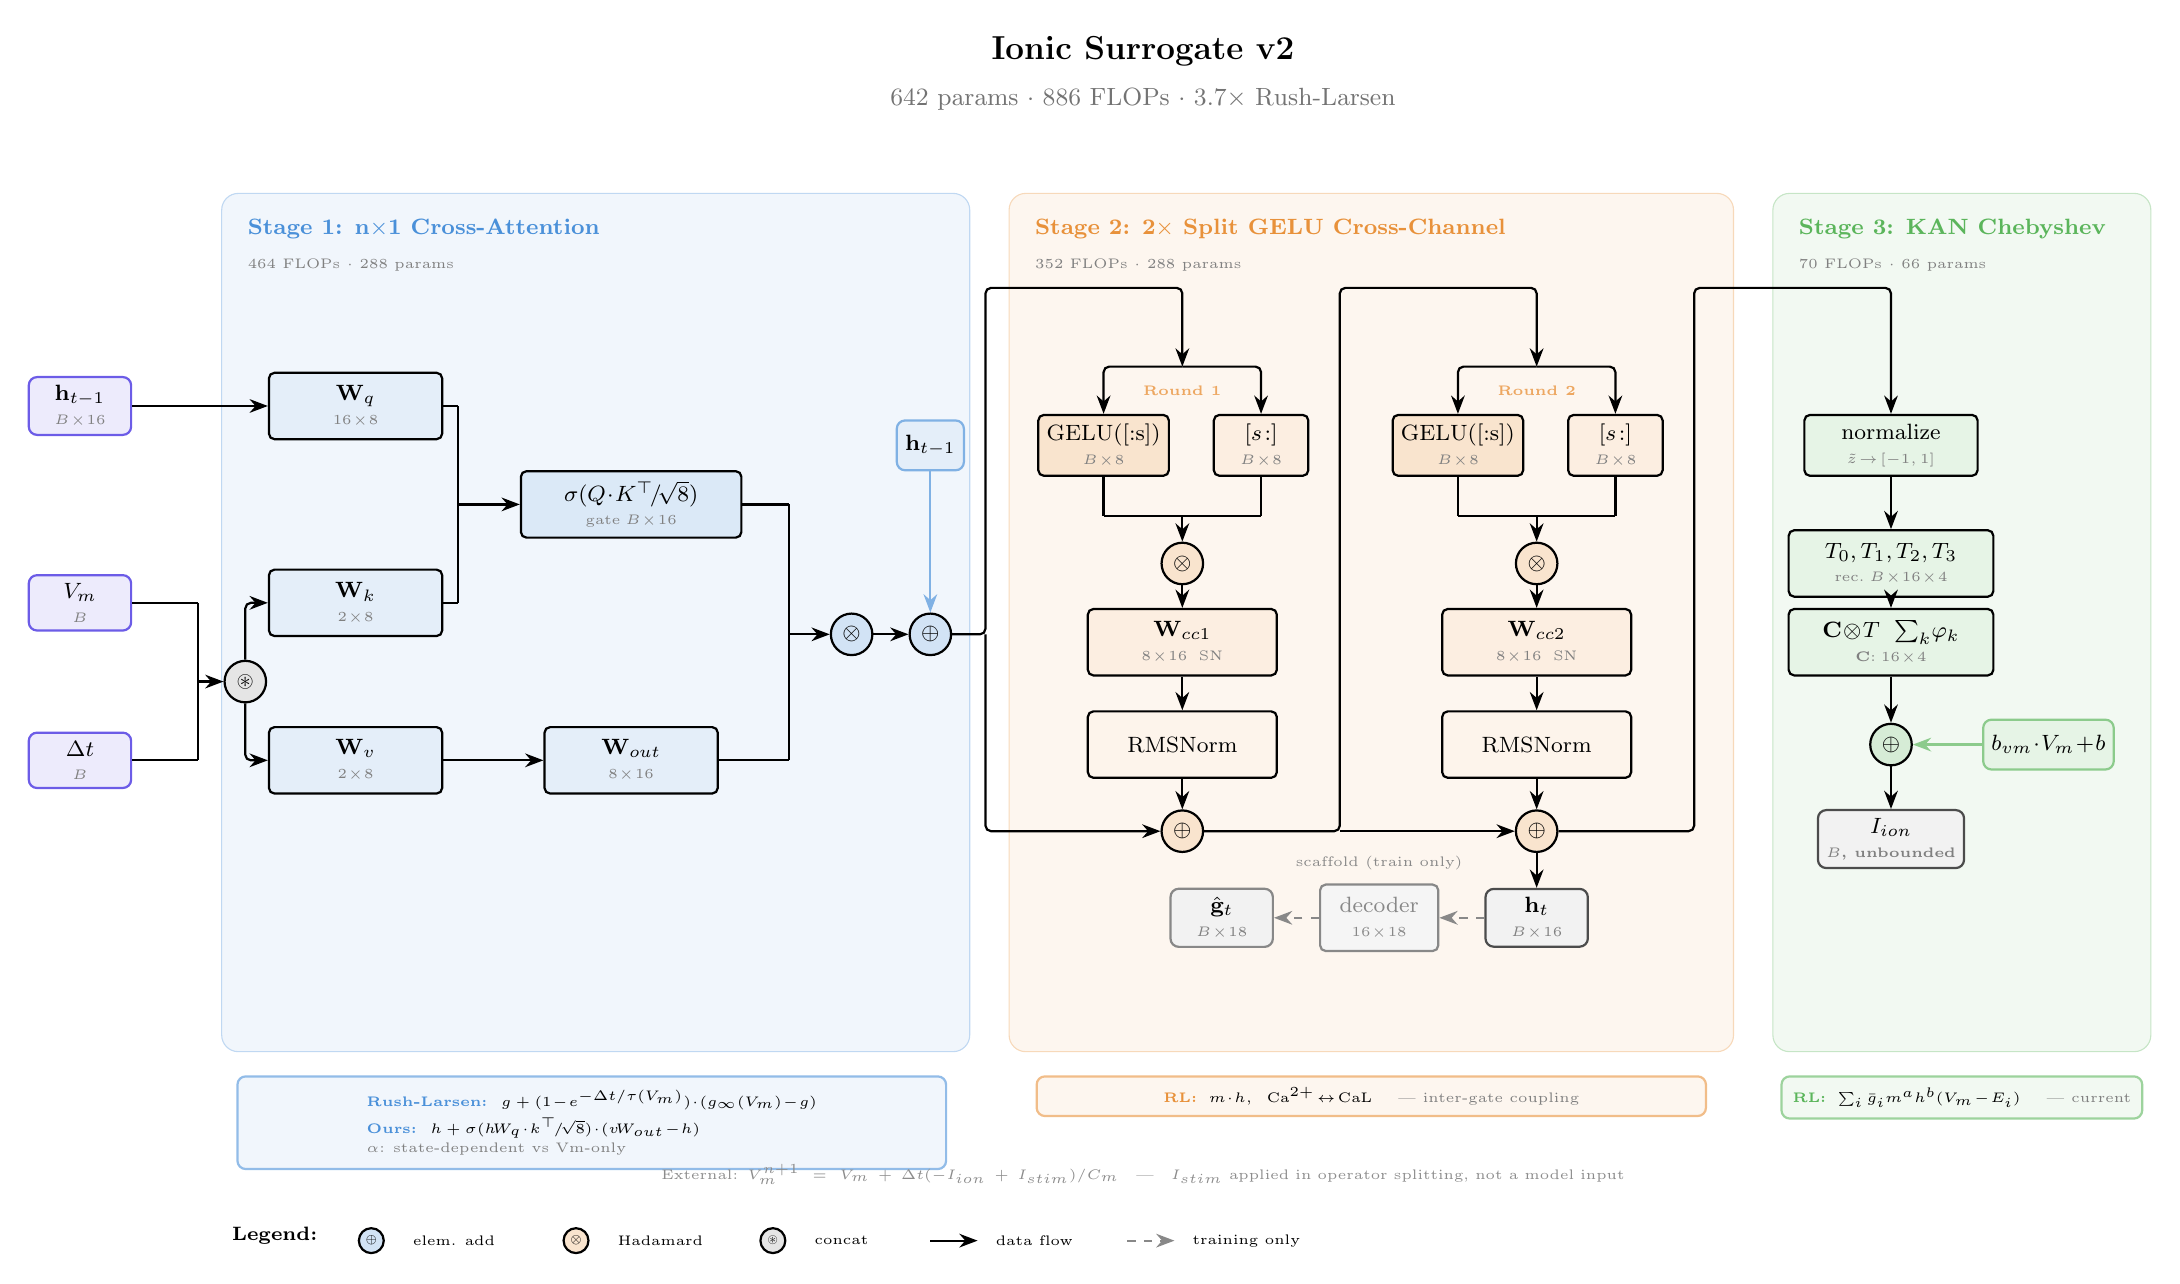
\begin{tikzpicture}[
    >=Stealth,
    line width=0.8pt,
    arrow/.style={->, rounded corners=2pt},
    dasharrow/.style={->, dashed, scaffold, rounded corners=2pt},
    layer/.style={
        rectangle, draw, rounded corners=2pt,
        minimum height=2.4em, minimum width=2.2cm,
        align=center, font=\footnotesize, inner sep=3pt
    },
    op/.style={
        circle, draw, inner sep=0pt,
        minimum size=1.5em, font=\footnotesize\bfseries
    },
    act/.style={
        rectangle, draw, rounded corners=2pt,
        minimum height=2.2em, minimum width=1.4cm,
        align=center, font=\footnotesize, inner sep=3pt
    },
    inputnode/.style={
        rectangle, draw=inputcol, rounded corners=3pt,
        fill=inputcol!12, minimum height=2em, minimum width=1.3cm,
        align=center, font=\footnotesize\bfseries, inner sep=3pt
    },
    outputnode/.style={
        rectangle, draw=black!70, rounded corners=3pt,
        fill=black!5, minimum height=2em, minimum width=1.3cm,
        align=center, font=\footnotesize\bfseries, inner sep=3pt
    },
    resinject/.style={
        rectangle, draw=#1!70, rounded corners=3pt,
        fill=#1!15, minimum height=1.8em,
        align=center, font=\footnotesize\itshape, inner sep=3pt
    },
    stagelab/.style={font=\footnotesize\bfseries, text=#1},
]

\def\boxtop{-0.3}
\def\boxbot{-11.2}
\def\routeY{-1.5}
\def\entryY{-2.5}

% =====================================================================
% TITLE
% =====================================================================
\node[font=\large\bfseries] at (12, 1.5) {Ionic Surrogate v2};
\node[font=\small, text=black!55] at (12, 0.9)
    {642 params $\cdot$ 886 FLOPs $\cdot$ 3.7$\times$ Rush-Larsen};

% =====================================================================
% INPUTS — all at x=-1.5
% =====================================================================
\node[inputnode] (latent) at (-1.5, -3.0) {$\mathbf{h}_{t-1}$\\[-1pt]{\tiny\color{black!50} $B\!\times\!16$}};
\node[inputnode] (vm) at (-1.5, -5.5) {$V_m$\\[-1pt]{\tiny\color{black!50} $B$}};
\node[inputnode] (dt) at (-1.5, -7.5) {$\Delta t$\\[-1pt]{\tiny\color{black!50} $B$}};

% Vm ⊛ Δt — merge bar then concat node
\coordinate (vmr) at (0.0, -5.5);
\coordinate (dtr) at (0.0, -7.5);
\draw (vm.east) -- (vmr);
\draw (dt.east) -- (dtr);
\draw (vmr) -- (dtr);
\coordinate (vdtmid) at (0.0, -6.5);
\node[op, fill=black!10] (cat) at (0.6, -6.5) {$\circledast$};
\draw[arrow] (vdtmid) -- (cat);

% =====================================================================
% STAGE 1: CROSS-ATTENTION (left → right)
% =====================================================================

\node[layer, fill=stage1!15] (wq) at (2.0, -3.0) {$\mathbf{W}_q$\\[-1pt]{\tiny\color{black!50} $16\!\times\!8$}};
\node[layer, fill=stage1!15] (wk) at (2.0, -5.5) {$\mathbf{W}_k$\\[-1pt]{\tiny\color{black!50} $2\!\times\!8$}};
\node[layer, fill=stage1!15] (wv) at (2.0, -7.5) {$\mathbf{W}_{v}$\\[-1pt]{\tiny\color{black!50} $2\!\times\!8$}};
\draw[arrow] (latent) -- (wq);
\draw[arrow] (cat) |- (wk.west);
\draw[arrow] (cat) |- (wv.west);

% Q+K merge → σ(Q·K^T/√8)
\coordinate (qr) at (3.3, -3.0);
\coordinate (kr) at (3.3, -5.5);
\draw (wq.east) -- (qr);
\draw (wk.east) -- (kr);
\draw (qr) -- (kr);
\coordinate (qkmid) at (3.3, -4.25);

\node[layer, fill=stage1!20, minimum width=2.8cm] (sigdot) at (5.5, -4.25)
    {$\sigma(Q\!\cdot\!K^\top\!/\!\sqrt{8})$\\[-1pt]{\tiny\color{black!50} gate\;$B\!\times\!16$}};
\draw[arrow] (qkmid) -- (sigdot);

\node[layer, fill=stage1!15] (wout) at (5.5, -7.5)
    {$\mathbf{W}_{out}$\\[-1pt]{\tiny\color{black!50} $8\!\times\!16$}};
\draw[arrow] (wv) -- (wout);

% gate+target merge → ⊗
\coordinate (gr) at (7.5, -4.25);
\coordinate (tr) at (7.5, -7.5);
\draw (sigdot.east) -- (gr);
\draw (wout.east) -- (tr);
\draw (gr) -- (tr);
\coordinate (gtmid) at (7.5, -5.9);

\node[op, fill=stage1!25] (had1) at (8.3, -5.9) {$\otimes$};
\draw[arrow] (gtmid) -- (had1);

% ⊕ with h_{t-1} from above
\node[op, fill=stage1!25] (add1) at (9.3, -5.9) {$\oplus$};
\draw[arrow] (had1) -- (add1);
\node[resinject=stage1] (res1) at (9.3, -3.5) {$\mathbf{h}_{t-1}$};
\draw[arrow, stage1!70] (res1) -- (add1);

% Stage 1 background
\begin{scope}[on background layer]
    \node[fit={(0.3,\boxtop)(9.8,\boxbot)}, fill=stage1!8, draw=stage1!35,
          rounded corners=6pt, inner sep=0pt] (s1bg) {};
\end{scope}
\node[stagelab=stage1, anchor=north west] at (0.5, -0.5)
    {Stage 1: n$\times$1 Cross-Attention};
\node[font=\tiny, text=black!50, anchor=north west] at (0.5, -1.0) {464 FLOPs $\cdot$ 288 params};

% =====================================================================
% ROUTING: Stage 1 → Round 1
% =====================================================================
\def\gapA{10.0}
\draw[arrow] (add1.east) -- (\gapA,-5.9) -- (\gapA,\routeY)
    -- (12.5,\routeY) -- (12.5,\entryY);

% =====================================================================
% STAGE 2: 2× SPLIT GELU (compressed)
% =====================================================================

% ---- ROUND 1 (center=12.5) ----
\node[font=\tiny\bfseries, text=stage2!80] at (12.5, -2.8) {Round 1};

\node[act, fill=stage2!25, minimum width=1.5cm] (gelu1) at (11.5, -3.5)
    {GELU([:s])\\[-1pt]{\tiny\color{black!50} $B\!\times\!8$}};
\node[act, fill=stage2!15, minimum width=1.2cm] (s1b) at (13.5, -3.5)
    {$[s\!:]$\\[-1pt]{\tiny\color{black!50} $B\!\times\!8$}};
\draw[arrow] (12.5,\entryY) -| (gelu1.north);
\draw[arrow] (12.5,\entryY) -| (s1b.north);

\coordinate (g1L) at (11.5, -4.4);
\coordinate (g1R) at (13.5, -4.4);
\draw (gelu1.south) -- (g1L);
\draw (s1b.south) -- (g1R);
\draw (g1L) -- (g1R);
\coordinate (g1mid) at (12.5, -4.4);
\node[op, fill=stage2!25] (had2a) at (12.5, -5.0) {$\otimes$};
\draw[arrow] (g1mid) -- (had2a);

\node[layer, fill=stage2!15, minimum width=2.4cm] (cc1) at (12.5, -6.0)
    {$\mathbf{W}_{cc1}$\\[-1pt]{\tiny\color{black!50} $8\!\times\!16$\; SN}};
\draw[arrow] (had2a) -- (cc1);

\node[layer, fill=stage2!10, minimum width=2.4cm] (rms1) at (12.5, -7.3)
    {RMSNorm};
\draw[arrow] (cc1) -- (rms1);

\node[op, fill=stage2!25] (add2a) at (12.5, -8.4) {$\oplus$};
\draw[arrow] (rms1) -- (add2a);
% Skip from Stage1→R1 routing junction
\draw[arrow] (\gapA,-5.9) -- (\gapA,-8.4) -- (add2a);

% ---- ROUTING: Round 1 → Round 2 ----
\def\gapB{14.5}
\draw[arrow] (add2a.east) -- (\gapB,-8.4) -- (\gapB,\routeY)
    -- (17.0,\routeY) -- (17.0,\entryY);

% ---- ROUND 2 (center=17.0) ----
\node[font=\tiny\bfseries, text=stage2!80] at (17.0, -2.8) {Round 2};

\node[act, fill=stage2!25, minimum width=1.5cm] (gelu2) at (16.0, -3.5)
    {GELU([:s])\\[-1pt]{\tiny\color{black!50} $B\!\times\!8$}};
\node[act, fill=stage2!15, minimum width=1.2cm] (s2b) at (18.0, -3.5)
    {$[s\!:]$\\[-1pt]{\tiny\color{black!50} $B\!\times\!8$}};
\draw[arrow] (17.0,\entryY) -| (gelu2.north);
\draw[arrow] (17.0,\entryY) -| (s2b.north);

\coordinate (g2L) at (16.0, -4.4);
\coordinate (g2R) at (18.0, -4.4);
\draw (gelu2.south) -- (g2L);
\draw (s2b.south) -- (g2R);
\draw (g2L) -- (g2R);
\coordinate (g2mid) at (17.0, -4.4);
\node[op, fill=stage2!25] (had2b) at (17.0, -5.0) {$\otimes$};
\draw[arrow] (g2mid) -- (had2b);

\node[layer, fill=stage2!15, minimum width=2.4cm] (cc2) at (17.0, -6.0)
    {$\mathbf{W}_{cc2}$\\[-1pt]{\tiny\color{black!50} $8\!\times\!16$\; SN}};
\draw[arrow] (had2b) -- (cc2);

\node[layer, fill=stage2!10, minimum width=2.4cm] (rms2) at (17.0, -7.3)
    {RMSNorm};
\draw[arrow] (cc2) -- (rms2);

\node[op, fill=stage2!25] (add2b) at (17.0, -8.4) {$\oplus$};
\draw[arrow] (rms2) -- (add2b);
% Skip from R1→R2 routing junction
\draw[arrow] (\gapB,-8.4) -- (add2b);

% ---- OUTPUTS from ⊕ ----

% DOWN → h_t
\node[outputnode] (hout) at (17.0, -9.5)
    {$\mathbf{h}_t$\\[-1pt]{\tiny\color{black!50} $B\!\times\!16$}};
\draw[arrow] (add2b.south) -- (hout);

% LEFT of h_t → decoder → ĝ_t (pointing left)
\node[layer, draw=scaffold, fill=scaffold!8, minimum width=1.5cm] (dec) at (15.0, -9.5)
    {\textcolor{scaffold}{decoder}\\[-1pt]{\tiny\color{scaffold} $16\!\times\!18$}};
\draw[dasharrow] (hout) -- (dec);
\node[outputnode, draw=scaffold] (gates) at (13.0, -9.5)
    {$\hat{\mathbf{g}}_t$\\[-1pt]{\tiny\color{black!50} $B\!\times\!18$}};
\draw[dasharrow] (dec) -- (gates);
\node[font=\tiny, text=scaffold, above=0.1em of dec] {scaffold (train only)};

% Stage 2 background — encompasses scaffold chain
\begin{scope}[on background layer]
    \node[fit={(10.3,\boxtop)(19.5,\boxbot)}, fill=stage2!8, draw=stage2!35,
          rounded corners=6pt, inner sep=0pt] (s2bg) {};
\end{scope}
\node[stagelab=stage2, anchor=north west] at (10.5, -0.5)
    {Stage 2: 2$\times$ Split GELU Cross-Channel};
\node[font=\tiny, text=black!50, anchor=north west] at (10.5, -1.0)
    {352 FLOPs $\cdot$ 288 params};

% =====================================================================
% STAGE 3: KAN CHEBYSHEV READOUT (center=21.5)
% =====================================================================

% Define norm3 FIRST so routing can target it
\node[act, fill=stage3!15, minimum width=2.2cm] (norm3) at (21.5, -3.5)
    {normalize\\[-1pt]{\tiny\color{black!50} $\tilde{z}\!\to\![-1,1]$}};

% ROUTING: Stage 2 → Stage 3 (single arrow, ends at norm3)
\def\gapC{19.0}
\draw[arrow] (add2b.east) -- (\gapC,-8.4) -- (\gapC,\routeY)
    -- (21.5,\routeY) -- (norm3);

\node[layer, fill=stage3!15, minimum width=2.6cm] (cheby) at (21.5, -5.0)
    {$T_0,T_1,T_2,T_3$\\[-1pt]{\tiny\color{black!50} rec.\;$B\!\times\!16\!\times\!4$}};
\draw[arrow] (norm3) -- (cheby);

\node[layer, fill=stage3!15, minimum width=2.6cm] (cprod) at (21.5, -6.0)
    {$\mathbf{C}\!\otimes\!T$\; $\sum_k\!\varphi_k$\\[-1pt]{\tiny\color{black!50} $\mathbf{C}$:\;$16\!\times\!4$}};
\draw[arrow] (cheby) -- (cprod);

% ⊕ centered on column, b_vm·Vm+b injects from right
\node[op, fill=stage3!25] (add3) at (21.5, -7.3) {$\oplus$};
\draw[arrow] (cprod) -- (add3);
\node[resinject=stage3, minimum width=1.5cm] (vmlocal) at (23.5, -7.3)
    {$b_{vm}\!\cdot\!V_m\!+\!b$};
\draw[arrow, stage3!70] (vmlocal) -- (add3);

\node[outputnode] (iion) at (21.5, -8.5)
    {$I_{ion}$\\[-1pt]{\tiny\color{black!50} $B$, unbounded}};
\draw[arrow] (add3) -- (iion);

% Stage 3 background
\begin{scope}[on background layer]
    \node[fit={(20.0,\boxtop)(24.8,\boxbot)}, fill=stage3!8, draw=stage3!35,
          rounded corners=6pt, inner sep=0pt] (s3bg) {};
\end{scope}
\node[stagelab=stage3, anchor=north west] at (20.2, -0.5)
    {Stage 3: KAN Chebyshev};
\node[font=\tiny, text=black!50, anchor=north west] at (20.2, -1.0)
    {70 FLOPs $\cdot$ 66 params};

% =====================================================================
% RUSH-LARSEN EQUIVALENT BOXES — below each stage, same color
% =====================================================================

% Stage 1 RL box
\node[rectangle, draw=stage1!60, fill=stage1!8, rounded corners=3pt,
      minimum width=9.0cm, align=left, font=\tiny, inner sep=5pt,
      anchor=north] (rl1) at (5.0, -11.5)
    {\textcolor{stage1}{\bfseries Rush-Larsen:}\;
     $g + (1\!-\!e^{-\Delta t/\tau(V_m)})\!\cdot\!(g_\infty(V_m)\!-\!g)$\\[2pt]
     \textcolor{stage1}{\bfseries Ours:}\;
     $h + \sigma(h\!W_q \!\cdot\! k^\top\!/\!\sqrt{8})\!\cdot\!(v\!W_{out}\!-\!h)$\\[1pt]
     \textcolor{black!50}{$\alpha$: state-dependent vs Vm-only}};

% Stage 2 RL box
\node[rectangle, draw=stage2!60, fill=stage2!8, rounded corners=3pt,
      minimum width=8.5cm, align=center, font=\tiny, inner sep=4pt,
      anchor=north] (rl2) at (14.9, -11.5)
    {\textcolor{stage2}{\bfseries RL:}\;
     $m \!\cdot\! h,\;\; \text{Ca}^{2+}\!\leftrightarrow\!\text{CaL}$
     \quad\textcolor{black!50}{--- inter-gate coupling}};

% Stage 3 RL box
\node[rectangle, draw=stage3!60, fill=stage3!8, rounded corners=3pt,
      minimum width=4.5cm, align=center, font=\tiny, inner sep=4pt,
      anchor=north] (rl3) at (22.4, -11.5)
    {\textcolor{stage3}{\bfseries RL:}\;
     $\textstyle\sum_i \bar{g}_i m^a h^b (V_m\!-\!E_i)$
     \quad\textcolor{black!50}{--- current}};

% External update
\node[font=\tiny, text=black!45, anchor=north, text width=14cm, align=center]
    at (12, -12.5)
    {External: $V_m^{n+1}\!=\!V_m + \Delta t(-I_{ion} + I_{stim})/C_m$
    \;\;---\;\; $I_{stim}$ applied in operator splitting, not a model input};

% =====================================================================
% LEGEND
% =====================================================================
\node[font=\scriptsize\bfseries, anchor=north west] at (0.3, -13.3) {Legend:};
\node[op, fill=stage1!25, scale=0.6] at (2.2, -13.6) {$\oplus$};
\node[font=\tiny, anchor=west] at (2.6, -13.6) {elem. add};
\node[op, fill=stage2!25, scale=0.6] at (4.8, -13.6) {$\otimes$};
\node[font=\tiny, anchor=west] at (5.2, -13.6) {Hadamard};
\node[op, fill=black!10, scale=0.6] at (7.3, -13.6) {$\circledast$};
\node[font=\tiny, anchor=west] at (7.7, -13.6) {concat};
\draw[arrow] (9.3,-13.6) -- ++(0.6,0);
\node[font=\tiny, anchor=west] at (10.0, -13.6) {data flow};
\draw[dasharrow] (11.8,-13.6) -- ++(0.6,0);
\node[font=\tiny, anchor=west] at (12.5, -13.6) {training only};

\end{tikzpicture}
\end{document}
